\begin{tikzpicture}[overlay, remember picture]
    \node[anchor=north west, rotate=0, gray, font=\tiny, text width=0.65\paperwidth] at (current page.south west)  [xshift=0, yshift=1cm] {
    [5] A. Elben et al., Statistical Correlations between Locally Randomized Measurements, Physical Review A 99, no. 5 (2019)
    };
\end{tikzpicture}

\vspace{-7mm}
The second Rényi entropy \vspace{-3mm}
\begin{equation*}
	S_2 (\rho_A) = - \log_2 \tr \rho_A^2.
\end{equation*}



Bipartite entanglement exists between subsystems $A$ and $B$ of $\mathcal{S}$  with reduced density matrices $\rho_A = \tr_{\mathcal{S}\backslash A} \rho$ and $\rho_B = \tr_{\mathcal{S}\backslash B} \rho$ \textbf{if}
\begin{equation*}
	S_2 (\rho_A) > S_2 (\rho_{AB}) \hspace{5 mm} \text{or} \hspace{5 mm}  
	S_2(\rho_B) > S_2 (\rho_{AB}).
\end{equation*}

\begin{minipage}{0.65\textwidth}

\vspace{-5mm}
\begin{figure}[h]
    \centering
    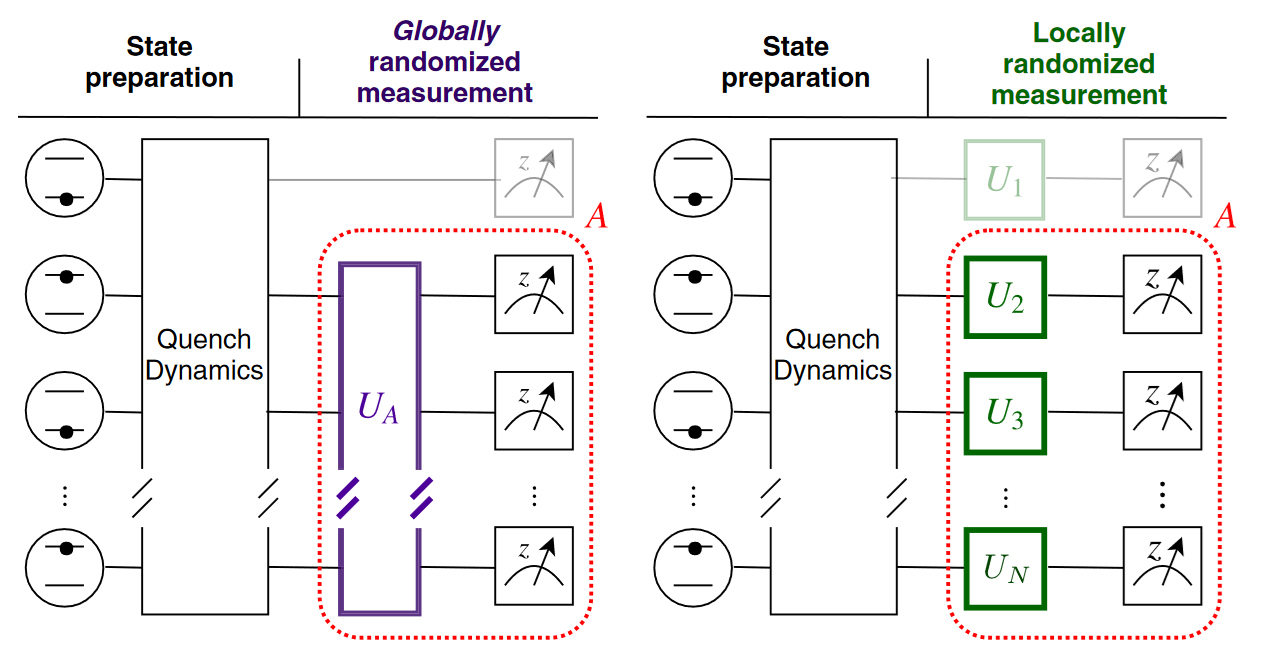
\includegraphics[width=\textwidth]{imgs/RU2.png}
    %\caption{}
    %\label{fig:}
\end{figure}


\end{minipage}
\hfill
\begin{minipage}{0.28\textwidth}
\begin{figure}[h]
    \centering
    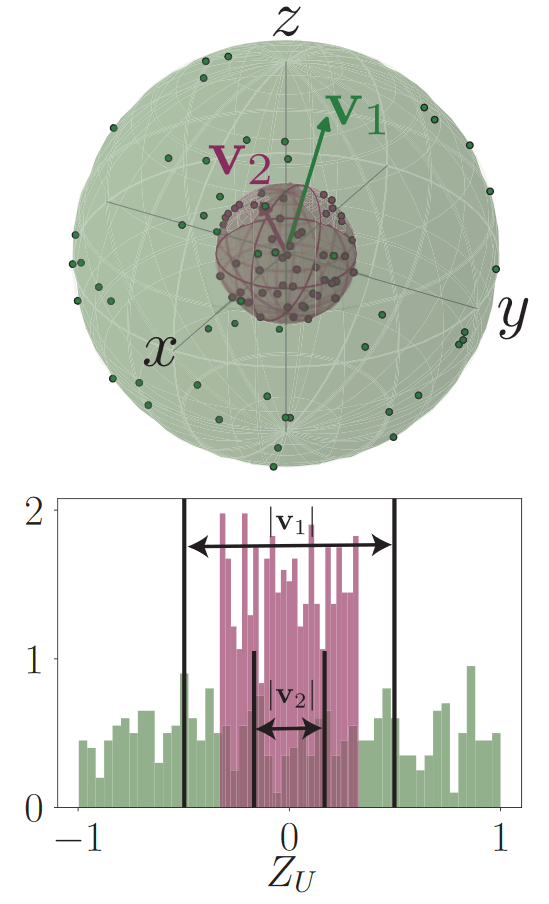
\includegraphics[width=\textwidth]{imgs/RU1.png}
    %\caption{}
    %\label{fig:}
\end{figure}
\end{minipage}


\onslide<2>{
\begin{tikzpicture}[overlay, remember picture]
    \fill[white,opacity=0.8] (current page.south west) rectangle (current page.north east);
    \node at (current page.center) {\usebeamerfont{title}\Huge\color{black} Thank you for your attention!};
\end{tikzpicture}
}